\documentclass[polish,polish,a4paper]{article}
\usepackage[utf8]{inputenc}
\usepackage[T1]{fontenc}
\usepackage[polish]{babel}
\usepackage{anysize}
\usepackage{siunitx}
\usepackage{graphicx}
\usepackage{listings}
\usepackage{pgfplots}
\usepackage{xcolor} % do komentarzy
\usepackage{diagbox} % macierz pomyłek
\usepackage{color, colortbl}
\usepackage{caption}
\usepackage{indentfirst}

\definecolor{Gray}{gray}{0.9}

\marginsize{2cm}{2cm}{1.5cm}{1.5cm}

\title{Elektroniczna karta pacjenta}
\author{Błażej Celmer (141197)\\Przemysław Ambroży (141182)}

\begin{document} 
	\maketitle

	\newpage
	
	\section{Wstęp}
		Celem projektu było stworzenie elektronicznej karty pacjenta, wykorzystującej standard FHIR do pobrania danych.
	
	\section{Technologia i wykorzystany serwer}
		Projekt został zrealizowany jako aplikacja webowa.
		Do jej stworzenia wykorzystaliśmy javascriptową bibliotekę \textbf{React}.
		Pomocne okazały się też paczki:
		\begin{description}
			\item[material-ui] -- interfejs użytkownika
			\item[chart.js] -- stworzenie wykresów
			\item[date-fns] -- manipulacja datami
		\end{description}

		Ze względu na niską jakość danych dostępnych na publicznym serwerze,
		skorzystaliśmy z własnego, uruchomionego lokalnie.
		Zaimportowaliśmy do niego dane kilkunastu pacjentów wygenerowanych w ramach projektu Synthea.
		Nie korzystaliśmy z żadnej biblioteki do obsługi standardu FHIR.
		Informacje zwrócone przez serwer interpretowaliśmy samodzielnie.
	
	\section{Interfejs użytkownika}
	
	\subsection{Lista pacjentów}
	
	\begin{figure}[!h]
		\centering
		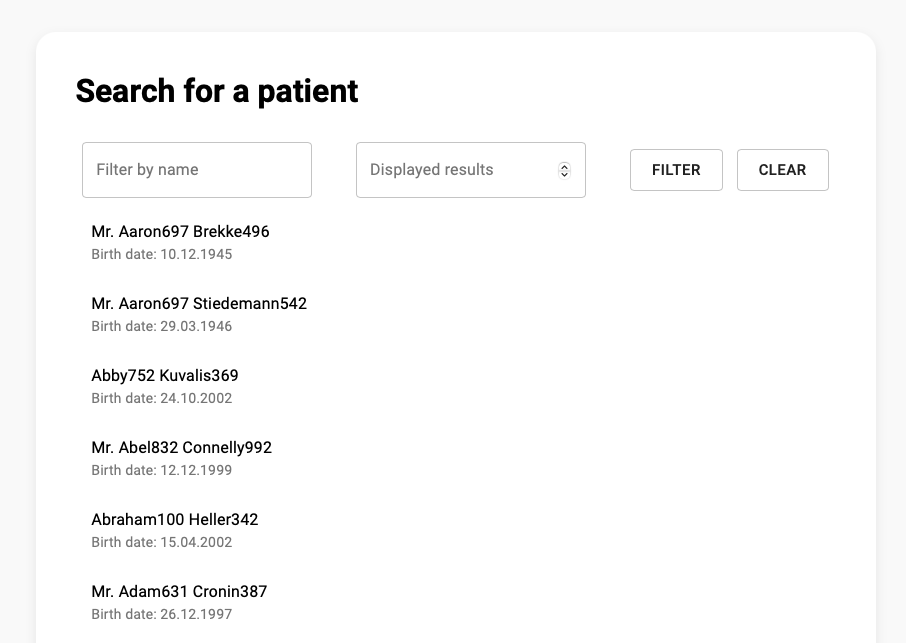
\includegraphics[width=.8\linewidth]{img/list1.png}
		\caption{Strona główna -- lista wszystkich pacjentów}
	\end{figure}
	Lista pacjentów umożliwia filtrowanie ich po imieniu i nazwisku,
	a także ograniczenie liczby wyświetlanych rezultatów.
	
	\begin{figure}[!h]
		\centering
		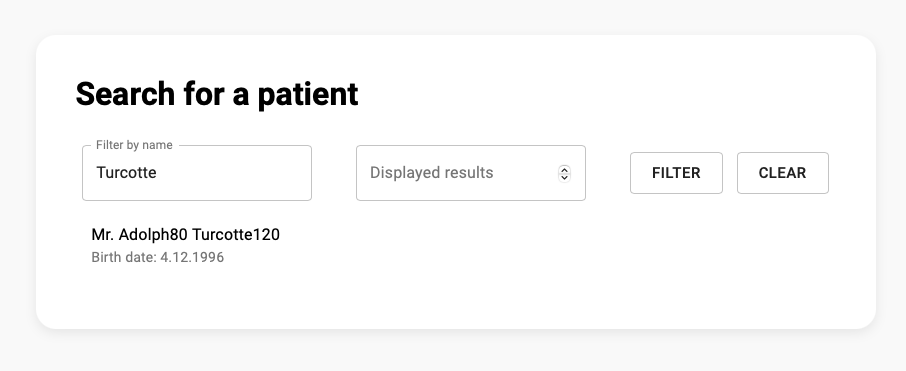
\includegraphics[width=.8\linewidth]{img/list2.png}
		\caption{Wyszukiwanie pacjentów po nazwisku}
	\end{figure}
	
	\newpage
	\subsection{Informacje o pacjencie}
	
	\begin{figure}[!h]
		\centering
		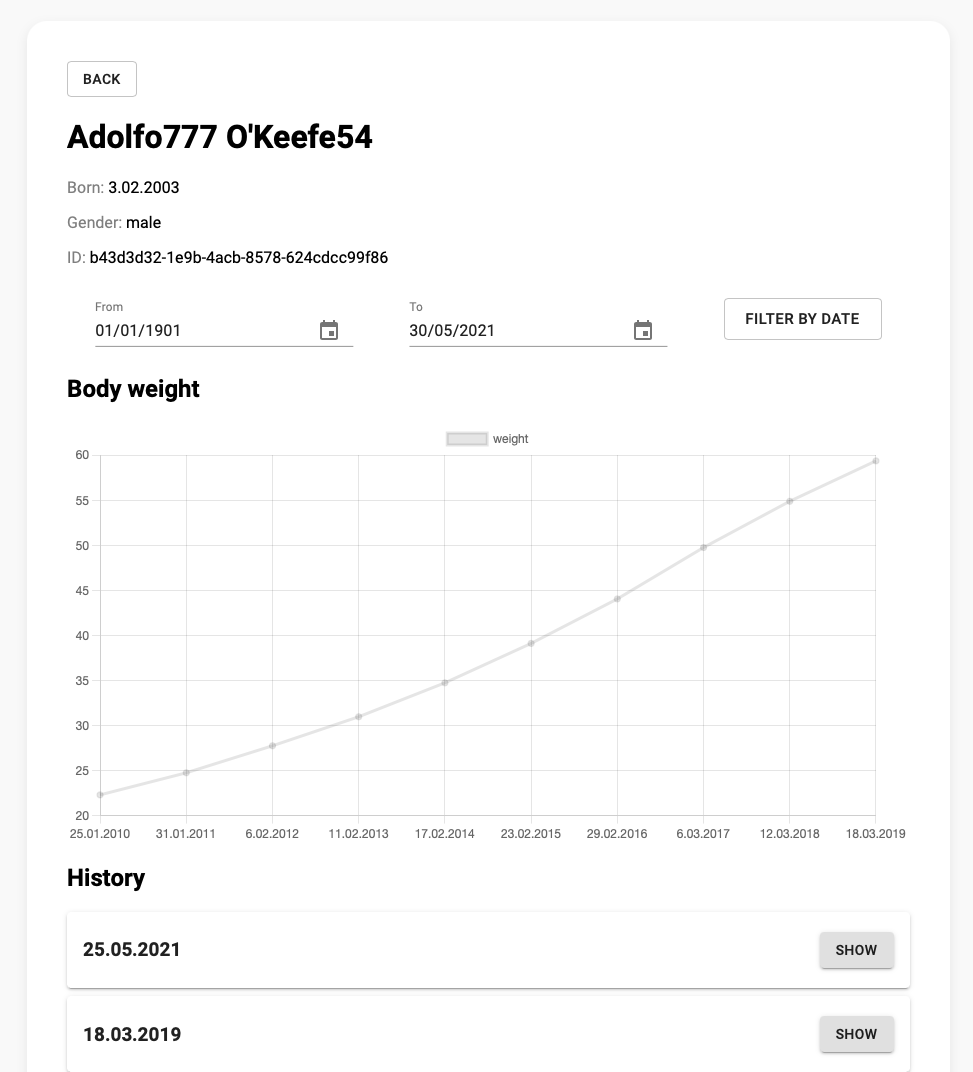
\includegraphics[width=.8\linewidth]{img/patient1.png}
		\caption{Strona z informacjami o pacjencie}
	\end{figure}
	
	\newpage
	
	\begin{figure}[!h]
		\centering
		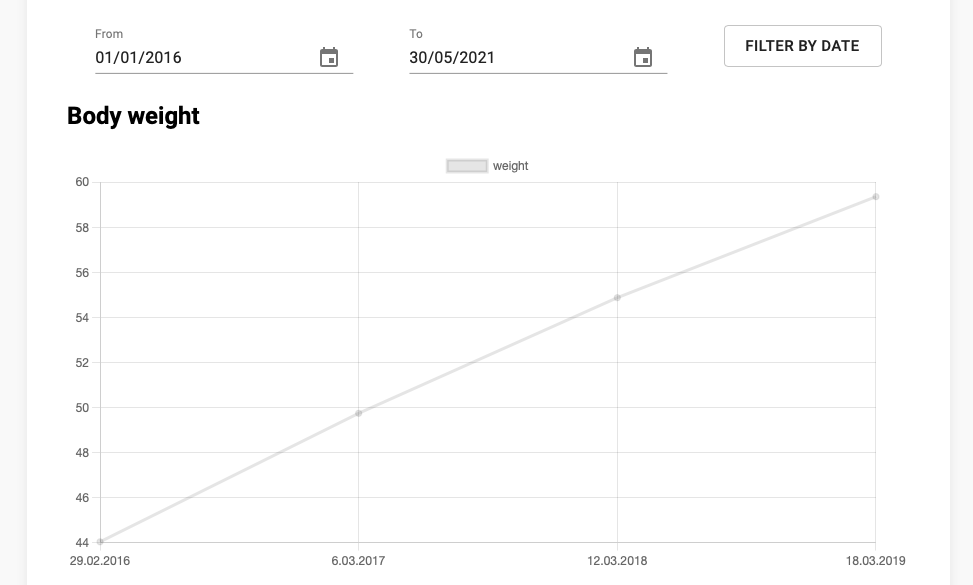
\includegraphics[width=.8\linewidth]{img/patient2.png}
		\caption{Filtrowanie wykresu z wagą pacjenta}
		\label{patient2}
	\end{figure}
	Zastosowany na rysunku \ref{patient2} filtr odnosi się zarówno do wykresu,
	jak i obserwacji i leków (widocznych niżej).
	
	\begin{figure}[!h]
		\centering
		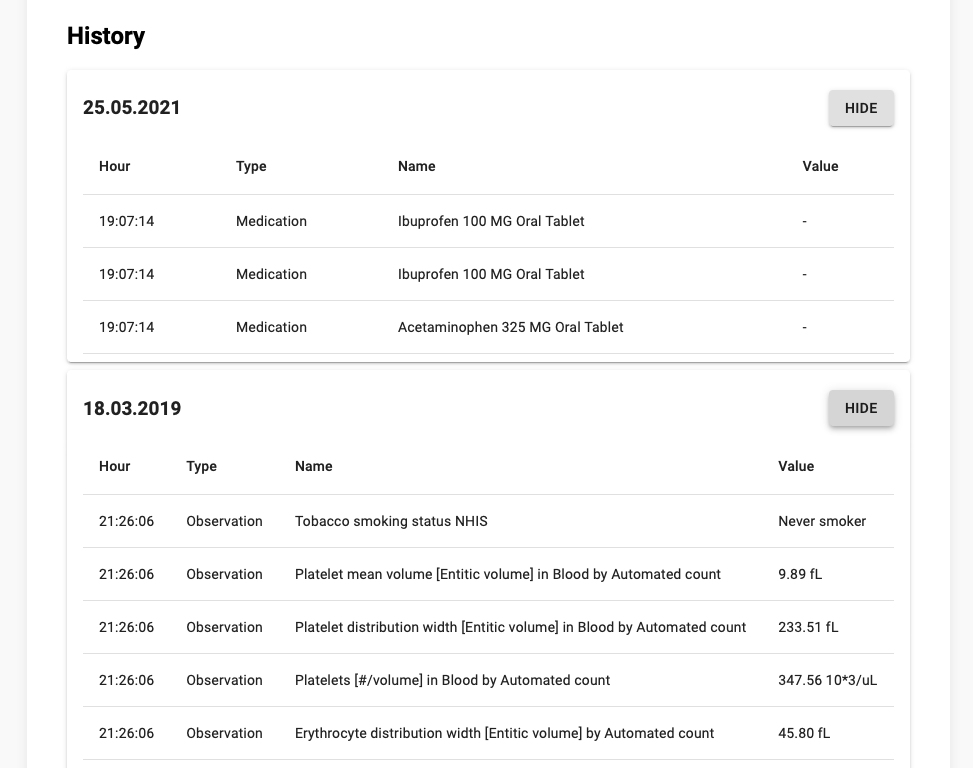
\includegraphics[width=.8\linewidth]{img/patient3.png}
		\caption{Historia obserwacji i przepisanych leków}
	\end{figure}
	
	Historia zawiera połączone dane dotyczące obserwacji oraz zażytych leków.
	Widok dzieli dane na poszczególne dni, zaczynając od najnowszych.
	Po rozwinięciu każdego, można zobaczyć listę wpisów tego dnia,
	zawierającą informacje o godzinie, typie wpisu, jego nazwie i ewentualnej zarejestrowanej wartości.
	
	\newpage
	
	\begin{figure}[!h]
		\centering
		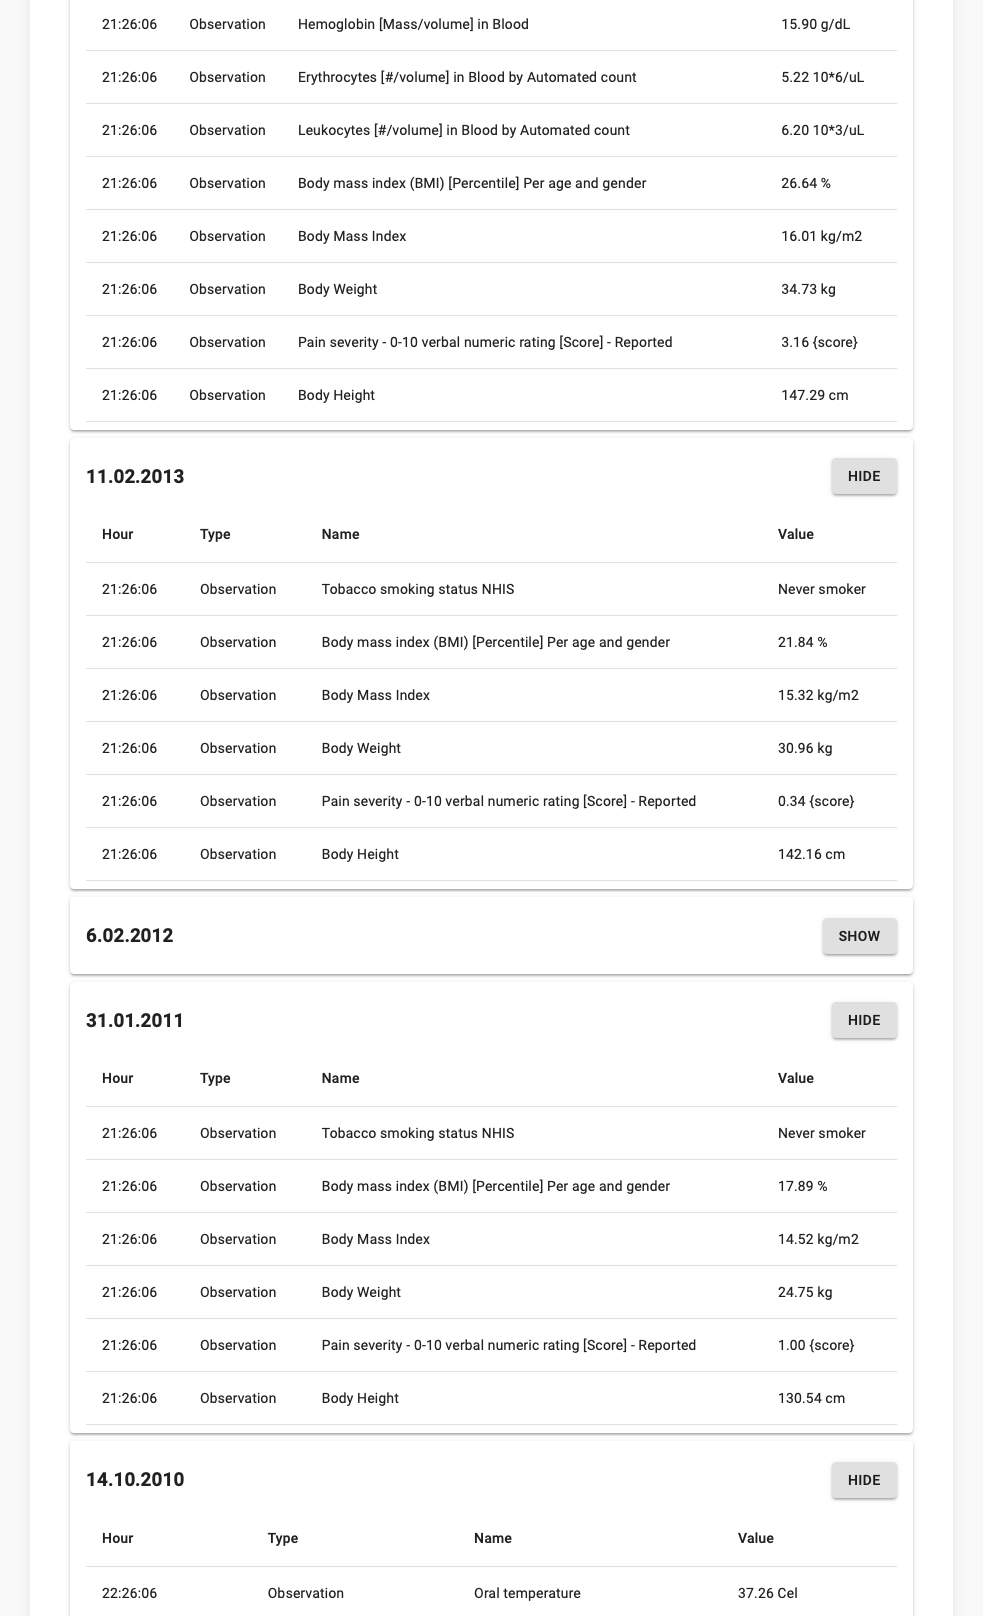
\includegraphics[width=.8\linewidth]{img/patient4.png}
		\caption{Wpisy w różnych dniach}
	\end{figure}

\end{document}